\subsection{Metrica bidimensionale}
Si studia la metrica
\[ g = \de s^2 = \frac{\epsilon \de x^2 + \de y^2}{y^2} \]
con \( \epsilon = \pm 1\).

\subsubsection*{Vettore di Killing} \todo
Considerando che la metrica non dipende dal modulo di x, ma solo da quello di y, si scrive immediatamente che per 
\[ \vec{k} = \left( \begin{array}{c}  cost \\ 0 \end{array}  \right) \]
\[ \mathcal{L}_{\vec{k}} g = 0 \]

\subsubsection*{Simboli di Christoffel}
L'azione di una particella libera, in parametrizzazione affine, si scrive
\[ S = \frac{1}{2} \int \de \lambda \frac{\epsilon \dot{x}^2 + \dot{y}^2}{y^2} \]
Le variazioni $\delta x$ portano a 
\[ \left(\frac{\epsilon \dot{x}}{y^2}\right)^\cdot = 0 \]
\[ \ddot{x} - \frac{2\dot{x}\dot{y}}{y} = 0 \]
mentre per $\delta y$ si ha
\[ \frac{\epsilon \dot{x}^2 + \dot{y}^2}{y^3} + \left(\frac{\dot{y}}{y^2}\right)^\cdot =0 \]
\[ \ddot{y} + \left(\frac{\epsilon \dot{x}}{y} - \frac{\dot{y}^2}{y} \right) =0 \]
Confrontando le'equazioni con la condizione per le geodetiche
\[ \ddot{x}^\mu + \Gamma^\mu_{\sigma\rho} \dot{x}^\sigma\dot{x}^\rho =0 \]
si trovano
\[ \Gamma^x_{xy} = \Gamma^x_{yx} = -\frac{1}{y} ; \;\;\; \Gamma^y_{xx} = \frac{\epsilon}{y} ; \;\;\; \Gamma^y_{yy} = - \frac{1}{y} \]
Ovvero
\begin{equation}
	\begin{pmatrix}
		\Gamma^x_{\; x} & \Gamma^x_{\; y} \\
		\Gamma^y_{\; x} & \Gamma^y_{\; y} 
	\end{pmatrix} = 
	\begin{pmatrix}
		-\frac{\de y}{y} 	& -\frac{\de x}{y}  \\
		\frac{\epsilon\de x}{y} & -\frac{\de y}{y} 
	\end{pmatrix}
\end{equation}
Con i simboli cos\`i trovati, si possono scrivere le seguenti equazioni
\begin{equation} 
	\begin{cases}
		\nabla e_x = -\frac{\de y}{y} \otimes e_x + \frac{e \de x}{y} \otimes e_y & \\ 
		\nabla e_y = -\frac{\de x}{y} \otimes e_x - \frac{\de y}{y} \otimes e_y & \\
	\end{cases}
\end{equation}

\subsubsection*{Tensore curvatura}
\[ R = \de\Gamma + \Gamma\wedge\Gamma \]
\begin{equation}
	(\de\Gamma)^i_j = \partial_\rho \Gamma_{\mu j}^i \dx^\rho \dx^\mu = \partial_y 
		\begin{pmatrix}
			0 & \frac{1}{y} \\
			-\frac{\epsilon}{y} & 0 \\
		\end{pmatrix}
		\dx\wedge\de y
\end{equation}
\[ (\Gamma\wedge\Gamma)^i_j = \Gamma^i_j\wedge\Gamma^j_k \]
e utilizzando il fatto che 
\[ \dx^\mu\wedge\dx^\mu = 0 = \dx^\mu\wedge\dx^\nu + \dx^\nu\wedge\dx^\mu \]
si trova che \( \Gamma\wedge\Gamma = 0 \).
Ne segue che 
\[ R = \frac{1}{y^2} 
	\begin{pmatrix}
		0 & -1 \\
		\epsilon & 0 \\
	\end{pmatrix}
	\dx\wedge\de y
\]
Il tensore di Ricci \`e 
\[ \mathrm{Ric}_{j\nu} = \delta^\mu_i R^i_{j\mu\nu} \]
E come matrice
\[ \mathrm{Ric} = 
	\begin{pmatrix}
		-\frac{\epsilon}{y^2} & 0 \\
		0                     & -\frac{1}{y^2} \\
	\end{pmatrix}
\]
Lo scalare di curvatura \`e definito come 
\[ R = g^{ij} R_{ij} \]
Si calcola $g^{ij}$ come inverso della metrica, da cui
\[ ||g^{ij}|| = \mathrm{diag}(\frac{y^2}{\epsilon}, y^2) \]
e $R=-2$.

\subsubsection*{Zweibein}
Scrivendo
\[ V^x = \frac{\dx}{y} \;\;\;\;\; V^y = \frac{\de y}{y} \;\;\;\;\; \eta_{ij} = 
	\begin{pmatrix}
		\epsilon & 0 \\
		0        & 1 \\
	\end{pmatrix}
\]
si ha
\[ \de s^2 = \eta_{ij} V^iV^j \]
\newline
Sapendo che 
\[ 	\begin{cases}
	\de V^x = \partial_y \left(\frac{1}{y}\right) \de y \wedge \dx & \\
	\de V^y = \partial_x \left(\frac{1}{y}\right) \dx \wedge \de y = 0  & \\
	\end{cases}
\]
e, considerando \(T^i = 0\), 
\[ \de V^i = -\omega^i_j\wedge V^j \]
(gli indici sono ora intesi nello spazio delle zweibein)
si trova
\[ \omega^y_x \wedge V^x = 0 \]
\[ \omega^x_y \wedge V^y = \frac{1}{y^2} \de y \wedge \dx \]
Considerando che, con la metrica piatta,
\[ V_i = \eta_{ij} V^j = \begin{cases}
	\epsilon V^i & \mathrm{se} \;\; i=x \\
	V^i	     & \mathrm{se} \;\; i=y \\
\end{cases} \]
si trova che 
\[ \omega^x_y \wedge V^y = -V^x\wedge V^y \]
da cui 
\[ \omega^x_y = -V^x \]
e naturalmente
\[ \omega^y_{\,x}= \epsilon\omega^{yx} = -\epsilon\omega^{xy} = -\epsilon\omega^x_{\,y} \]
che verifica la condizione trovata per $\de V^y$.
L'antisimmetria di $\omega^i_{\;j}$ si trasferisce a $R^i_{\;j}$, che avr\`a non nulli solo
\[ R^x_{\;y} = \de \omega^i_{\;j} = -V^x\wedge V^y \;\;\;\;\; R^y_{\;x} = -\epsilon\de \omega^i_{\;j} = \epsilon V^x\wedge V^y \]
Pertanto 
\[ R = \begin{pmatrix}
		0 & -1 \\
		\epsilon & 0 \\
	\end{pmatrix} V^x \wedge V^y \]
Il tensore di Ricci ha componenti
\[ \mathrm{Ric}_{ij} = 
	\begin{pmatrix}
		R^y_{x|yx} & R^x_{x|xy} \\
		R^y_{y|yx} & R^x_{y|xy} \\
	\end{pmatrix}
	= \begin{pmatrix}
		R^x_{\;y} & 0 \\
		0 & R^x_{\;y} \\
	\end{pmatrix}
	= \begin{pmatrix}
		-\epsilon & 0 \\
		0 & -1 \\
	\end{pmatrix}
\]
per cui lo scalare 
\[ R = g^{ij} \mathrm{Ric}_{ij} = -\epsilon^2 -1=-2 \]

\subsubsection*{Derivate covarianti}
I vettori tangenti alle Zweibein sono quelli tali per cui
\[ e_i(V^j) = \delta_i^j \]
e sono pertanto
\[ e_x = y \dx \;\;\;\;\; e_Y = y\de y \]
Se ne calcolano le derivate covarianti, con connessione $\omega^i_{\;j}$:
\begin{equation} \label{eq:der_vettori}
	\nabla e_x = \omega^y_{\;x} e_y = \epsilon e_y \otimes V^x \;\;\;\;\; \nabla e_y = \omega^x_{\;y} e_x =  e_x \otimes V^x 
\end{equation}



\subsubsection*{Integrali primi}
Gli integrali primi
\[ \begin{cases}
	p_x = \frac{\dot{x}}{y^2} & \\
	\sigma = \frac{\epsilon\dot{x}^2 + \dot{y}^2}{y^2} & \\
  \end{cases}
\]
danno le condizioni
\[ \begin{cases}
	\dot{x} = p_x y^2 & \\
	\dot{y}^2 = (\sigma - \epsilon p_x^2 y^2 ) y^2 & \\
  \end{cases}
\]
Si procede calcolando
\[ \left(\frac{\de v}{\dx}\right)^2 = \left( \frac{\de v}{\de \lambda} \frac{\de \lambda}{\dx}  \right)^2 
	= \left( \frac{2\dot{y}y}{\dot{x}} \right)^2 \]
e, sostituendo le condizioni trovate con gli integrali primi, si ottiene
\[ \left(\frac{\de v}{\dx}\right)^2 = \frac{4}{p_x^2} (\sigma - \epsilon\dot{x}^2 y^2 )\]

Per integrare questa equazione,
\[ \frac{\de v}{\dx} = \frac{2}{p_x}\sqrt{\sigma - \epsilon p_x^2 v} \;\;\; \Rightarrow \;\;\;
	\frac{2\sqrt{\sigma}}{p_x} \dx = \frac{\de v}{ \sqrt{1 - \frac{\epsilon p_x^2 v}{\sigma}}} \]
Si sostituisce al secondo membro 
\[ v \rightarrow q = \frac{\epsilon p_x^2 v}{\sigma} \;\;\;\Rightarrow\;\;\; 
	\frac{\sigma}{\epsilon p_x^2} \frac{\de q}{\sqrt{1-q}} \]
Un'ulteriore sostituzione porta a 
\[ q \rightarrow \theta=\arcsin{\sqrt{q}} \;\;\;\Rightarrow\;\;\;
	\frac{2\sigma}{\epsilon p_x^2} \de{\cos\theta} \]
Pertanto, tenendo conto che 
\[ \cos\arcsin\sqrt{q} = \sqrt{1-q} \]
l'integrazione porta a 
\[ \frac{p_x\epsilon}{\sqrt{\sigma}}(x-x_0) = \sqrt{1-\frac{\epsilon p_x^2 v}{\sigma}} -c_0 \]
che raccogliendo le costanti e riarrangiando porta a 
\[ (p_x \epsilon x - K)^2 = \sigma - \epsilon p_x^2v \]
Al variare di $\epsilon$ e $\sigma$, si ottengono i seguenti grafici:
\begin{figure}[htbp]
 \centering
 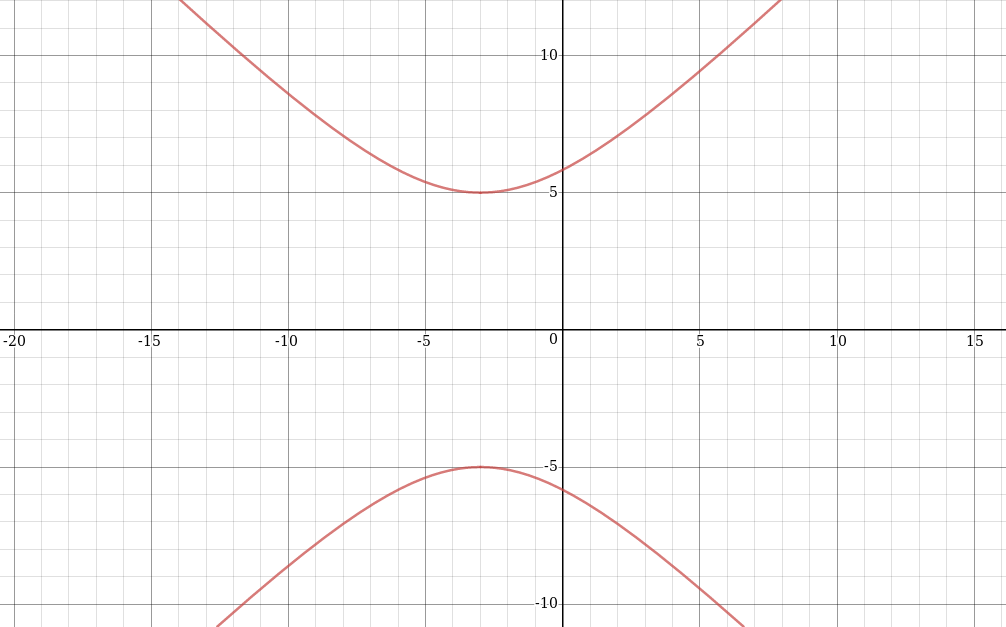
\includegraphics[width=\textwidth]{images/foglio3_neg_neg}
	\caption*{\(\epsilon=-1, \;\sigma=-1\)}
 \label{figure:neg_neg}
\end{figure}
\begin{figure}[htbp]
 \centering
 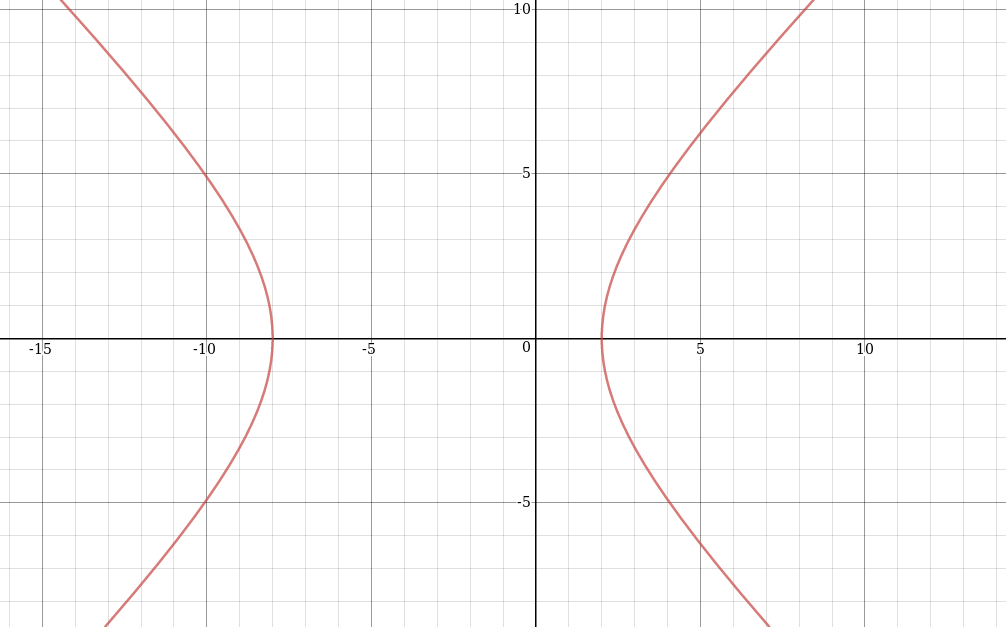
\includegraphics[width=\textwidth]{images/foglio3_pos_neg}
	\caption*{\(\epsilon=-1, \;\sigma=+1\)}
 \label{figure:pos_neg}
\end{figure}
\begin{figure}[htbp]
 \centering
 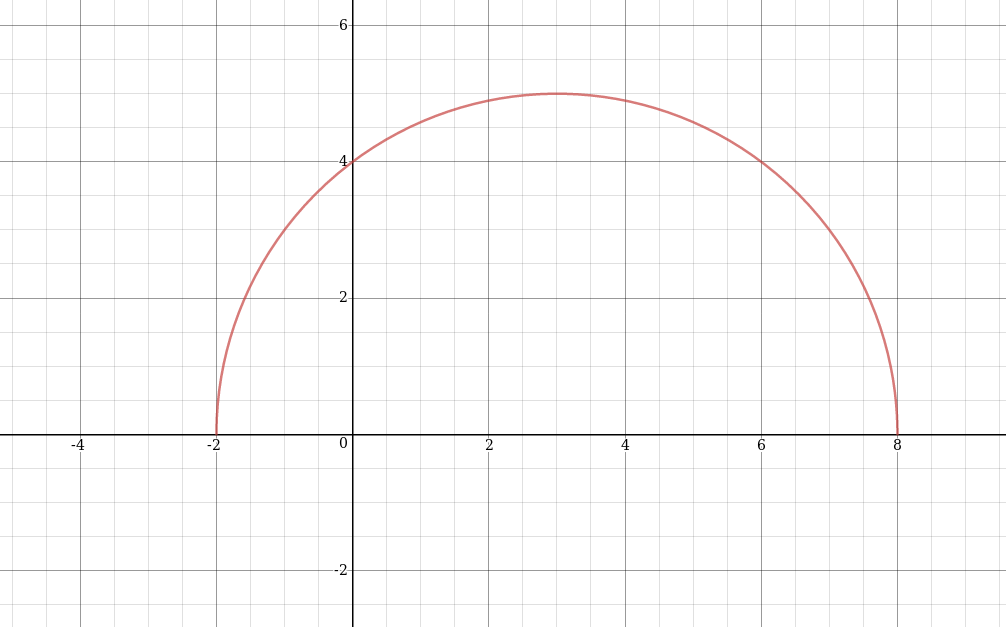
\includegraphics[width=\textwidth]{images/foglio3_pos_pos}
	\caption*{\(\epsilon=+1, \;\sigma=+1\)}
 \label{figure:pos_pos}
\end{figure}

\subsubsection*{Derivata di un campo vettoriale}
\[ \nabla X = (\nabla X^i) \partial_i + X^i \nabla\partial_i \]
dove 
\[ \nabla X^i = \partial_j X^i \dx^j = \de X^i \]
e utilizzando la \ref{eq:der_vettori}
\[ \nabla X = (\de X^x - X^yV^x) e_x + (\de X^y + \epsilon X^x V^x) e_y \]


\subsubsection{Traiettoria circolare}
Presa la traiettoria
\[ \gamma(t) = (x_0 + r\cos\omega t, y_0 + r\sin\omega t) \]
si considera il trasporto parallelo lungo essa, scrivibile come
\[ \nabla_{\dot{\gamma}} X = \gamma \rfloor \nabla X = 0 \]
Sviluppando questa condizione si trova (per brevit\`a: i simboli $\cos$ e $\sin$ sottintendono l'argomento $\omega t$; si scrive $y$ intendendolo valutato su $\gamma$, come indicato a pedice))
\[ \begin{cases}
	\dot{\gamma}^\mu (\nabla_\mu X)^x = \omega r \left[ -\sin \partial_x X^x + \cos \partial_y X^x
		+\frac{\sin X^y - \cos X^x}{y}\right]_\gamma = 0  & \\
	\dot{\gamma}^\mu (\nabla_\mu X)^y = \omega r \left[ -\sin \partial_x X^y + \cos \partial_y X^y
		+\frac{-\epsilon\sin X^x - \cos X^y}{y}\right]_\gamma = 0  & \\
   \end{cases}
\]
Prendendo \(\epsilon=+1\), moltiplicando membro a membro la seconda equazione per $i$ e sommando le due si trova
\[\omega r\left[(-\sin \partial_x+\cos \partial_y)(X^x+ix^y) - \left.\frac{1}{y}\right|_\gamma (X^x+iX^y) e^{+\omega t}\right] = 0 \]
Definendo \( Z = X^x +iX^y \), \(\dot{Z} = \dtotal{\gamma^i}{t}\left.\nabla_i Z \right|_\gamma\) e l'equazione diventa
\[ \dot{Z} - \omega r \frac{e^{i\omega t}}{y_0 + r\sin{\omega t}} Z \]
